

\documentclass[A4paper,twoside,twocolumn]{article}

\usepackage{float}
\usepackage{graphicx}
\usepackage{subfigure}
\usepackage[sc]{mathpazo} % Use the Palatino font
\usepackage[T1]{fontenc} % Use 8-bit encoding that has 256 glyphs
\linespread{1.05} % Line spacing - Palatino needs more space between lines
\usepackage{microtype} % Slightly tweak font spacing for aesthetics

\usepackage[english]{babel} % Language hyphenation and typographical rules

\usepackage[left=1.5cm,right=1.5cm,top=2.5cm,bottom=2.5cm]{geometry} % Document margins
\usepackage[hang, small,labelfont=bf,up,textfont=it,up]{caption} % Custom captions under/above floats in tables or figures
\usepackage{booktabs} % Horizontal rules in tables

\usepackage{lettrine} % The lettrine is the first enlarged letter at the beginning of the text

\usepackage{enumitem} % Customized lists
\setlist[itemize]{noitemsep} % Make itemize lists more compact

\usepackage{abstract} % Allows abstract customization
\renewcommand{\abstractnamefont}{\normalfont\bfseries} % Set the "Abstract" text to bold
\renewcommand{\abstracttextfont}{\normalfont\small\itshape} % Set the abstract itself to small italic text

\usepackage{titlesec} % Allows customization of titles
\renewcommand\thesection{\Roman{section}} % Roman numerals for the sections
\renewcommand\thesubsection{\roman{subsection}} % roman numerals for subsections
\titleformat{\section}[block]{\large\scshape\centering}{\thesection.}{1em}{} % Change the look of the section titles
\titleformat{\subsection}[block]{\large}{\thesubsection.}{1em}{} % Change the look of the section titles

\usepackage{fancyhdr} % Headers and footers
\pagestyle{fancy} % All pages have headers and footers
\fancyhead{} % Blank out the default header
\fancyfoot{} % Blank out the default footer
\fancyhead[C]{} % Custom header text
\fancyfoot[RO,LE]{\thepage} % Custom footer text

\usepackage{titling} % Customizing the title section

\usepackage{hyperref} % For hyperlinks in the PDF

%----------------------------------------------------------------------------------------
%	TITLE SECTION
%----------------------------------------------------------------------------------------

\setlength{\droptitle}{-4\baselineskip} % Move the title up

\pretitle{\begin{center}\Huge\bfseries} % Article title formatting
\posttitle{\end{center}} % Article title closing formatting
\title{Is it better to build multi-language Stackoverflow site?} % Article title
\author{%
\normalsize Australian National University \\ % Your institution
\normalsize \href{mailto:u5870997@anu.edu.com}{u5870997@anu.edu.com} % Your email address
%\and % Uncomment if 2 authors are required, duplicate these 4 lines if more
%\textsc{Jane Smith}\thanks{Corresponding author} \\[1ex] % Second author's name
%\normalsize University of Utah \\ % Second author's institution
%\normalsize \href{mailto:jane@smith.com}{jane@smith.com} % Second author's email address
}
\date{\today} % Leave empty to omit a date
\renewcommand{\maketitlehookd}{%
\begin{abstract}



\end{abstract}
}

%----------------------------------------------------------------------------------------

\begin{document}

% Print the title
\maketitle

%----------------------------------------------------------------------------------------
%	ARTICLE CONTENTS
%----------------------------------------------------------------------------------------

\section{Introduction}


%------------------------------------------------

\section{Contents}

\begin{itemize}
\item Link
\item User
\item Post
\item Tag
\end{itemize}

%------------------------------------------------

\section{Link}
This part of work is based on the links of stackoverflow and Russian stackoverflow. According to the previous results by some other similar research, links are good proof to present the user activity and community activity. Combine the amount of links and the activities of link between these two communities can provide some evidence for the necessity of a multi-language sub site. First of all, we need to find out how many posts and comments used links, and how many people links there evidence in their answers and questions. Then the analysis would be presented in some charts to show the results. 
\\Currently, there are 34,857,917 posts and 55,852,373 comments in Stackoverflow site while 280,424 posts and 499,186 comments in Russian Stackoverflow subsite. Basically, they are devided into two sets, one is the set of posts and comments who use links to stackoverflowcom and the other is those to ru.stackoverflow.com. Some statistics are presented in figures below.
\\For the posts and comments in Stackoverflow:
	\begin{figure}[H]
		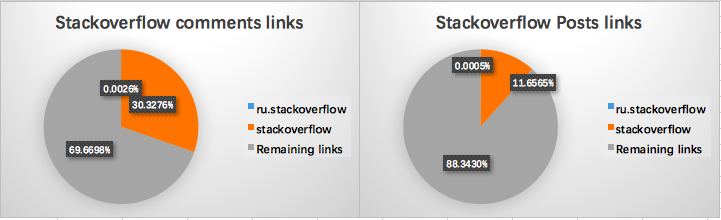
\includegraphics[width = 0.4\textwidth]{link3.png}
		\caption{Links in Stackoverflow}
  	\end{figure}
Similarly, for Russian Stackoverflow:
	\begin{figure}[H]
		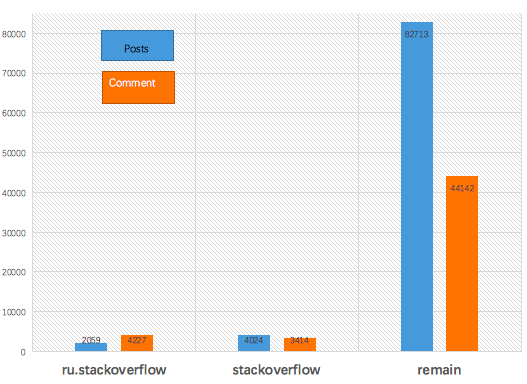
\includegraphics[width = 0.4\textwidth]{link1.png}
		\caption{Amount of links activily in Russian Stackoverflow}
		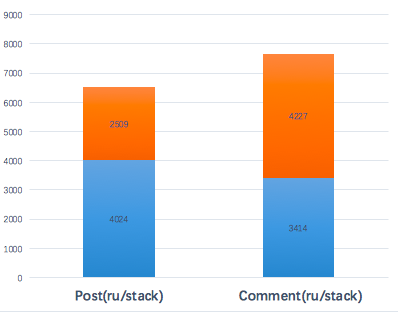
\includegraphics[width = 0.4\textwidth]{link2.png}
		\caption{Compare betweenthe amount of links to stackoverflow site and Russian subsite}
  	\end{figure}
Apparetly, in stackoverflow set, 12,220,205 posts used links in their body text. 11.66\% of them link to stackoverflow itself, while only 67 links are lead to Russian subsite. In Russian stackoverflow, 88,796 posts used links in theis body text. 4.53\% of them link to stackoverflow main site, while 2.32\% of them link to Russian subsite itself. The result of the link activities shows that Russian Stackoverlfow subsite is relatively independent community, which support itself by a lot of link activities instead of making the majority of their references to the main Stackoverflow site. However, in some ways the Russian Stackoverflow subsite has a non-negligible demand of knowledge refenrence to the main site according to the compare of destination between the amount of links.
		
\section{Users}
It has been widely believed that users data is highly important for the community analysis. User activity can be revealed by data, which have already been structurized into different types. Hence, the analysis of user would be expanded with different aspects.
\\First of all, the intersection of these two sets is the foundation of this part of research, which is the users that owns th main site account and Russian subsite account at the same time. A point worth mentioning is that not only people from Russia use Russian for introduction and answers, but also some other countries like Ukraine and Belarus. That is the user base called "Russian Speakers".
\\Stackoverflow main site has 6,833,276 users, while Ru.stackoverflow has 65,623 users art the same time. Each stackexchange user account has a unique accountId, which is always the same if the user sign up for a subsite account like Russian or Spanish Stackoverflow. Using this information, the number of the intersection can be found as 35,751, which is nearly 54.48\% of the total number of users in Russian Stackoverflow. 

\subsection{CreationDate}
Focusing on this intersection user base, the user movement is calculated by their account creation date of each site. As the result shows in figure 4, 11,253 people have their Russian Stackoverflow account first and then sign up for a Stackoverflow account. While the other 24,498 users are the opposite of them. On the one hand, user base is segregated by the new subsite and the number of users leaving the main site to their native language subsite is growing with the time goes by.  On the other hand, when 3 out of 10 users flow to Stackoverflow from Russian Stackoverflow, the otehr 7 of these 10 people flow to Russian stackoverflow from Stackoverflow,which means Russian site suprisingly offers a lot of users as feedback to Stackoverflow.
	\begin{figure}[H]
		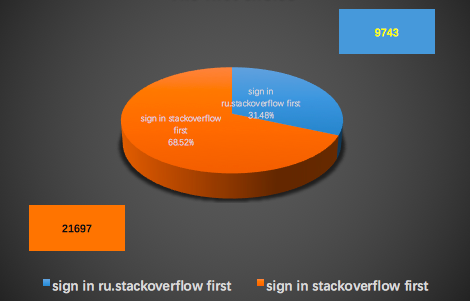
\includegraphics[width = 0.4\textwidth]{user2.png}
		\caption{Creation date compare}
	\end{figure}
Here is the statistics for the users sign up Russian Stackoverflow in figure 5. 
	\begin{figure}[H]
		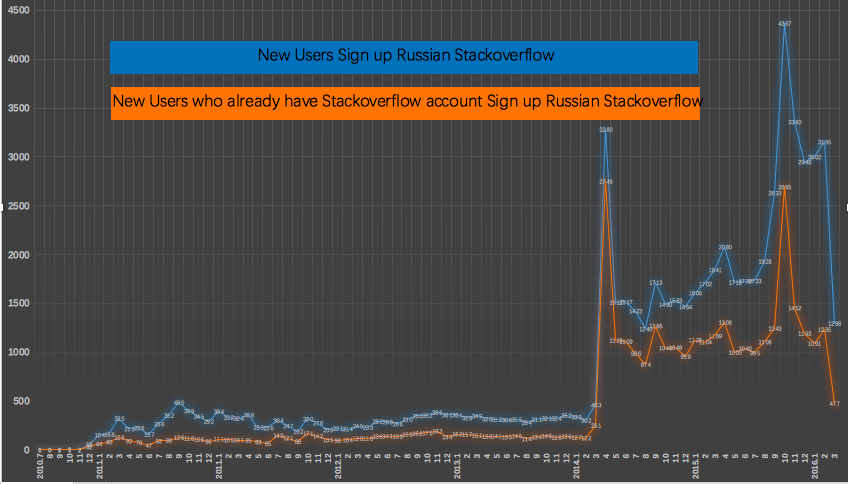
\includegraphics[width = 0.4\textwidth]{user1.png}
		\caption{User movement for signing up Russian Stackoverflow in each month}
  	\end{figure}

\subsection{Location and AboutMe}
Basically, all the users who can speak Russian can be found in a simple way. The Russian Alphabet can filter all the people using Russian in their DIsplayname or self introduction of the main Stackoverflow account.  In this way, 19,300 users can be seen as a set. Surprisingly, only 3,946 of them have a Russian stackoverflow account, which means 79.55\% of these Russian speakers choose to use Stackoverflow site only.
There are not a pretty huge number of users use their native language, which is Russian, in Stackoverflow site. And compare this number with the total number of Russian Stackoverflow user base, it is still not a big number. The conclusion is that  the majority of Russian Speakers prefer to use English as the only general language on the main site, and the fragmenting level is slight.

\subsection{Reputation}
Reputation is a very valuable information that can be used to reveal the active level of users. The assumption is the user whose reputation is under 20 will be seen as an inactive user. As the result shows in figure 6, a huge number of inactive users, which includes a number of barely used accounts whose reputation is 1. 
	\begin{figure}[H]
		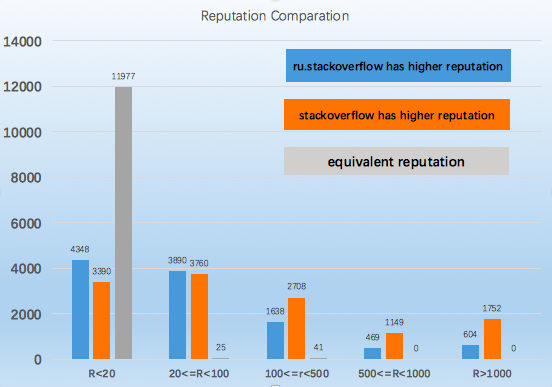
\includegraphics[width = 0.4\textwidth]{user3.png}
		\caption{Reputation compare}
  	\end{figure}
And the remaining data shows there are more users' stackoverflow account owns a higher reputation than their Russian ones. Only 8,360 users in the 31,440 overlapping set have a over 100 reputation in either of their accounts, and in those 24,498 users who migrated from Stackoverflow to Russian Stackoverflow 6,489 users have a over 100 reputation, which means they are active users. 
%==============

\section{Post}

Generally, for each single community, core user groups are the foudation because of their contribution like a large number of posts and comments. Similarly, in figure 7, for the 65623 overlapping users, we can simply get a group of core user by calculating their posts. For the Russian users, simply calculating their post count and the results are presented in figure 8. This result is very consistent with the twenty-eight law, that is, about twenty percent of the user made a contribution of about eighty percent
	\begin{figure}[H]
		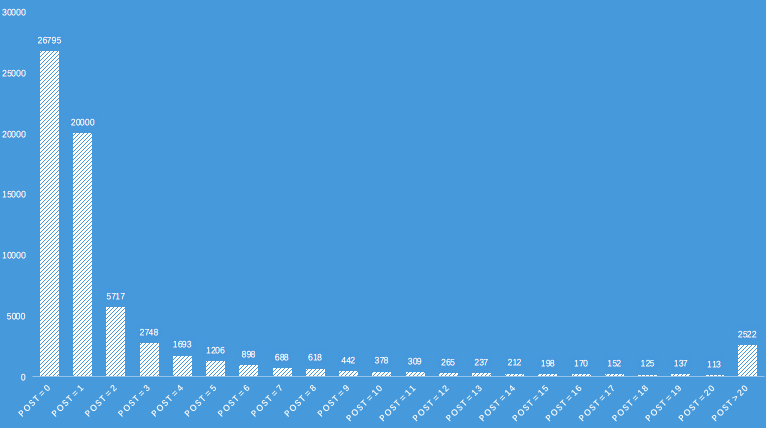
\includegraphics[width = 0.42\textwidth]{coreuser.png}
		\caption{russian users posts count result}
  	\end{figure}
So we can see that 4818 users who contributed more than 10(can equal) posts own 237,557 posts, which is almost 76.8\% of the total amount of Russian posts. So it is better to make an assumption that these kind of users are the core users for the Russian sub site. On the other hind,s we need to use their creation date again to defenite their direction of migration between these two sites, which is showed in figure 9.
 \begin{figure}[H]
		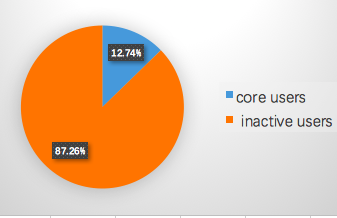
\includegraphics[width = 0.42\textwidth]{coreuser1.png}
		\caption{Core users that owns both Stackoverflow account and Russian Stackoverflow account at the same time}
		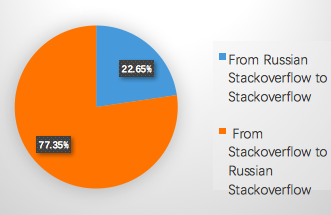
\includegraphics[width = 0.42\textwidth]{coreuser2.png}
		\caption{The compare of migration drection }
  	\end{figure}
As the results above, 1845 out of 11253 overlap users who migrated to Stackoverflow, which is 16.40\% are proved still be core users in Russian stackoverflow site, while 1402 out of overlap 24498 users who migrated from Stackoverflow, which is 5.72\% are proved to be core users.
There are and 310,539 posts in Russian Stackoverflow, and 237,557 posts in Russian Stackoverflow are contributed by the core user group that owns 4818 people. In other words, the 7.34\% core users contribute 76.50\% of the total posts in Russian Stackoverflow.

For the 1402 core users who already have Stackoverflow account before thier creation of Russian Stackoverflow account, the compare between the post activities before their migration with the post activities after their migration can definitly reveal their emphasized aspect.	The idea is that the object of reference of the users it themselve. To compare the post frequency before and after they create a new subsite account, which called user migration.
	\begin{displaymath}
	f(x)=\frac{PostCountAfterMigration/TimeLengthAfterMigration  }{  PostCountBeforeMigration /TimeLengthBeforeMigration}	 			\end{displaymath}
Briefly, for all the Russian users, the result of their active proportion is in figure 10.We can see no matter which domain we choose, it cannot change the trend of the user active ratio. The main trend is linear increasing.
 \begin{figure}[H]
 		\centering 
	\subfigure[A general figure for all users] { \label{fig:b} 
	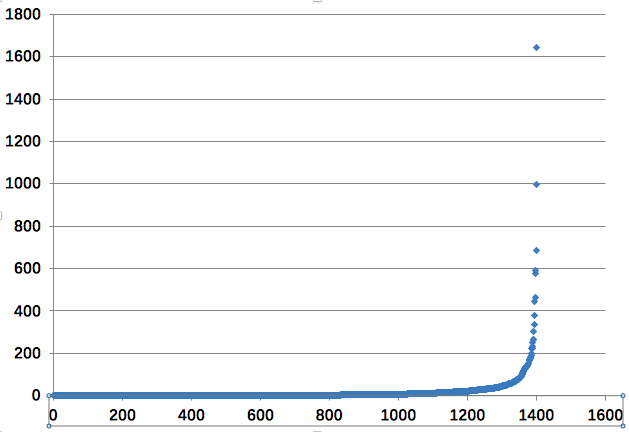
\includegraphics[width=0.99\columnwidth]{ratiochart1.png} 
	}
	\subfigure[Active ratio close to 1 ] { \label{fig:b} 
	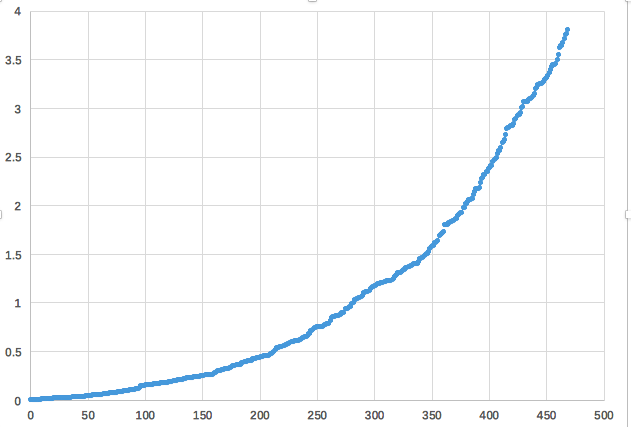
\includegraphics[width=0.99\columnwidth]{ratiochart2.png} 
	}  
	\caption{active ratio chart}
	\label{fig} 
  	\end{figure}


\subsection{PostCount}
As the result in figure 10, we can easily determine that 0.9~1.1 is the domain of fair activity area. So there are three level of activity, the first one is active, which means the count of users' post is abov 1.1 mutiple of their previous one. The second one is fair, which is between 0.9 and 1.1. The third one is inactive, which is under 0.9. The result is in figure 11.
	\begin{figure} [H]
	\centering 
	\subfigure[Russian Post Activity.] { \label{fig:a} 
	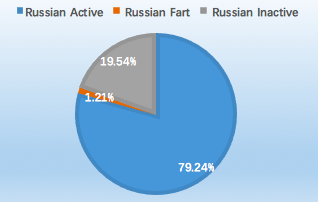
\includegraphics[width=0.7\columnwidth]{test1.png} 
	} 
	\subfigure[StackOverflow Post Activity.] { \label{fig:b} 
	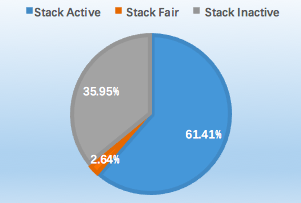
\includegraphics[width=0.7\columnwidth]{test2.png} 
	}
	\subfigure[Total Post Activity.] { \label{fig:b} 
	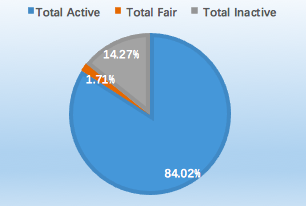
\includegraphics[width=0.7\columnwidth]{test3.png} 
	}  
	\caption{ User Post Activity Result. } 
	\label{fig} 
	\end{figure}
And the in these 1402 users who own both Stackoverflow account and Russian Stackoverflow account and migrated from Stackoverflow site to Russian sub site. 861 of them are both on both sites after their migration, and 3 of them are fair, while 200 of them are inactive. The result is in figure 12.
	\begin{figure}[H]
		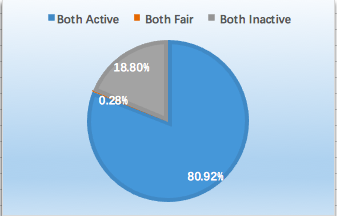
\includegraphics[width = 0.42\textwidth]{useractivity_post2.png}
		\caption{Overall result}
  	\end{figure}
  	
  	
  	
\begin{figure} [H]
	\centering 
	\subfigure[Russain Stackoverflow Active.] { \label{fig:a} 
	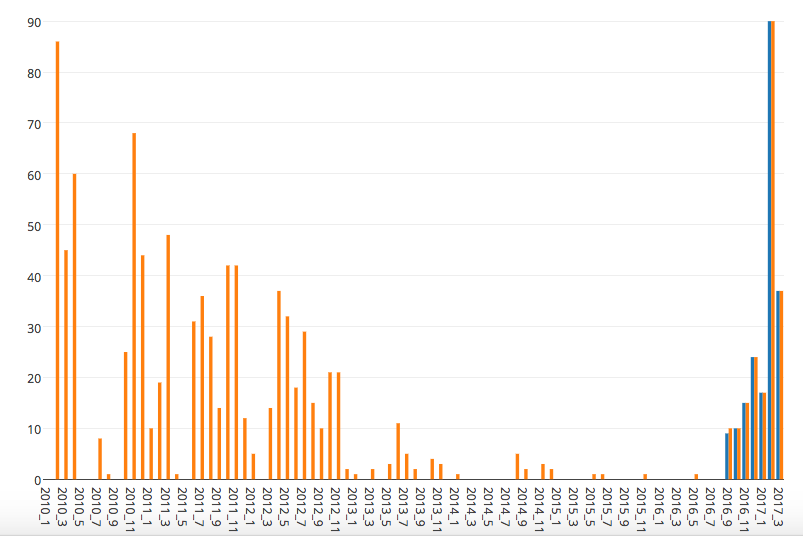
\includegraphics[width=0.7\columnwidth]{example1.png} 
	} 
	\subfigure[Russain Stackoverflow Inactive.] { \label{fig:b} 
	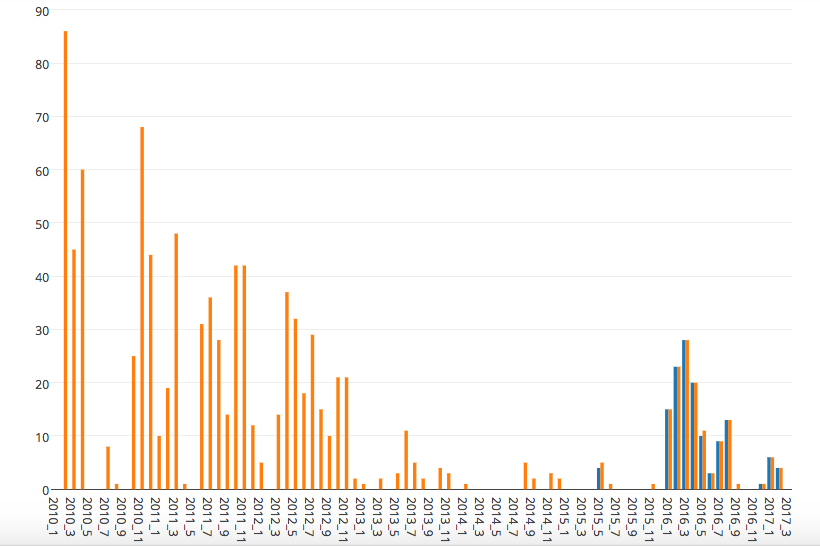
\includegraphics[width=0.7\columnwidth]{example2.png} 
	}
	\subfigure[Stackoverflow Activite.] { \label{fig:b} 
	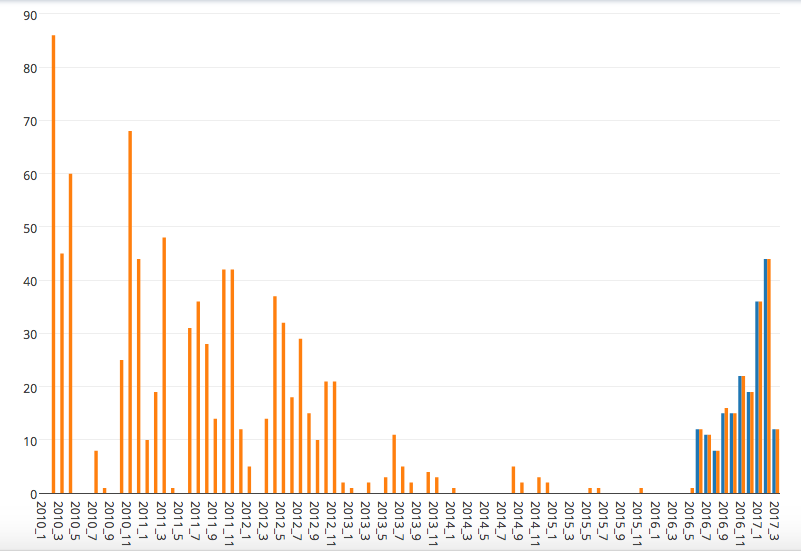
\includegraphics[width=0.7\columnwidth]{example3.png} 
	}  
	\subfigure[Stackoverflow Inactive.] { \label{fig:a} 
	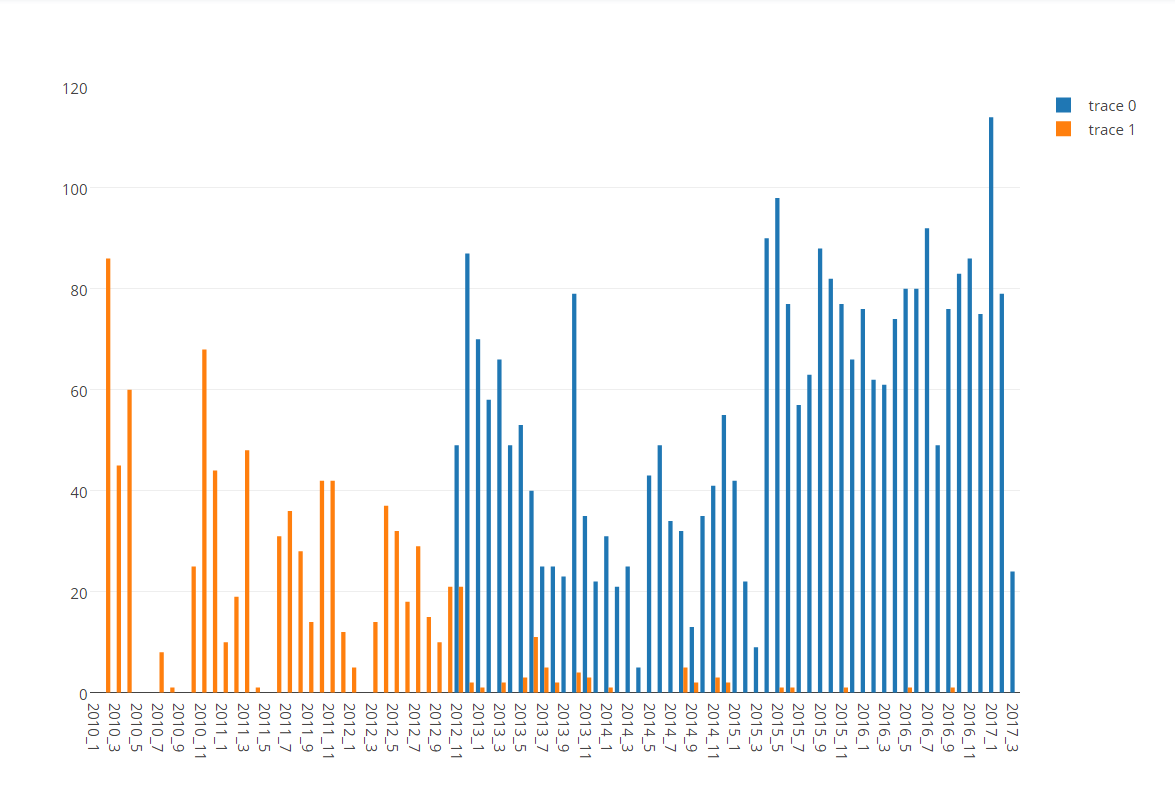
\includegraphics[width=0.7\columnwidth]{example4.png} 
	} 
	\caption{ 8 examples(Part 1) } 
	\label{fig} 
	\end{figure}
\begin{figure} [H]
	\centering 
	\subfigure[Total Active.] { \label{fig:b} 
	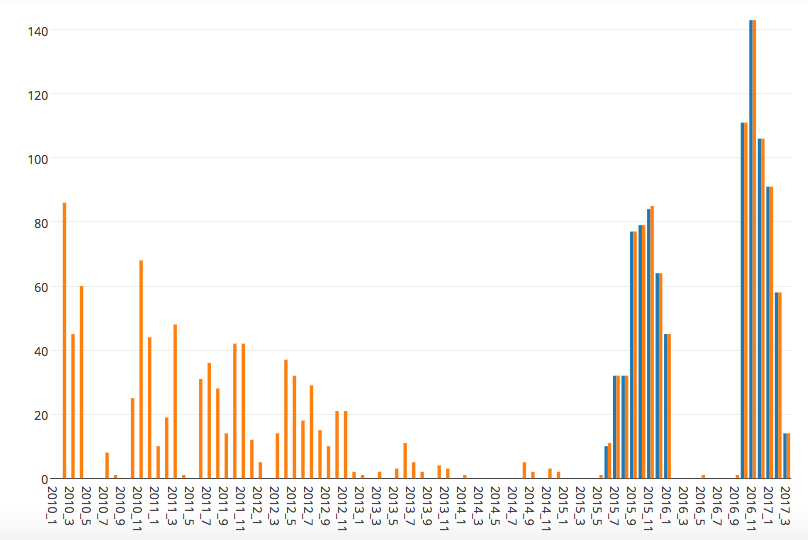
\includegraphics[width=0.7\columnwidth]{example6.png} 
	}
	\subfigure[Total Inactive.] { \label{fig:b} 
	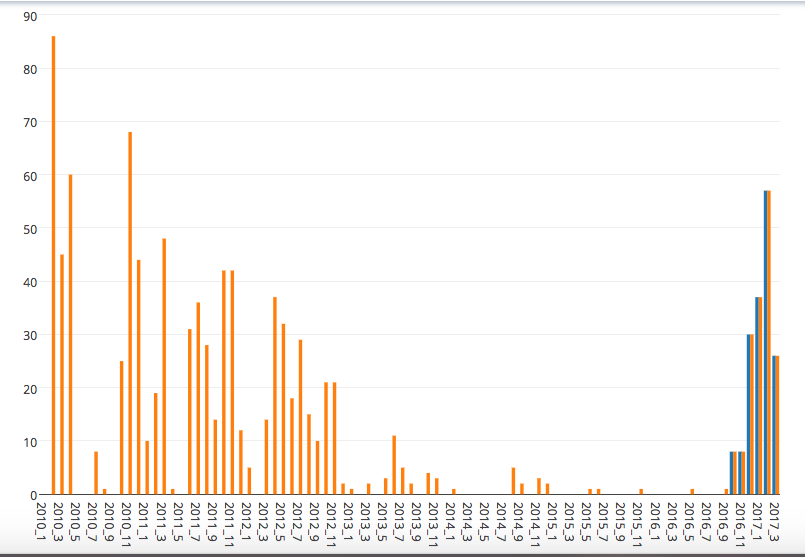
\includegraphics[width=0.7\columnwidth]{example5.png} 
	}  
	\subfigure[Both Active.] { \label{fig:a} 
	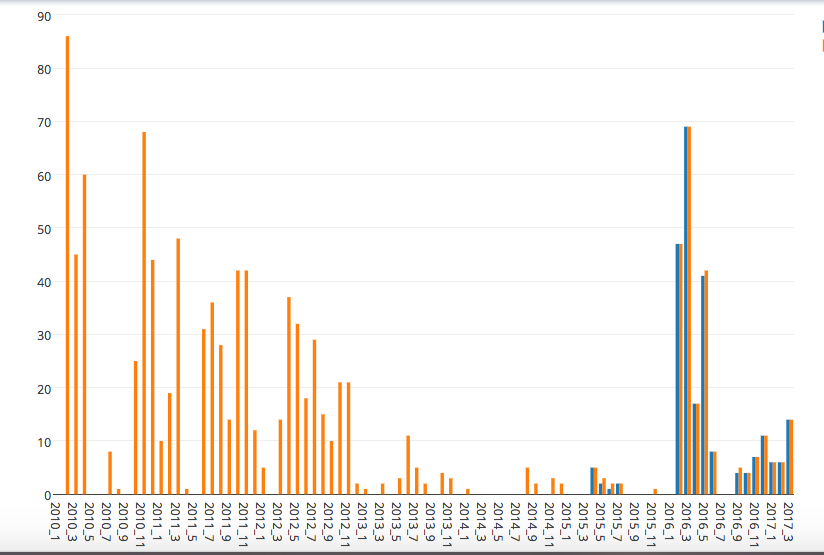
\includegraphics[width=0.7\columnwidth]{example7.png} 
	} 
	\subfigure[Both Inactive.] { \label{fig:b} 
	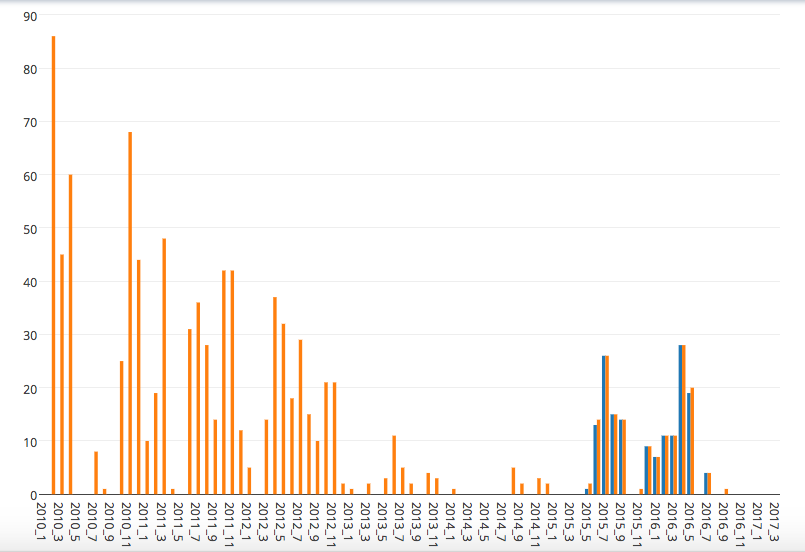
\includegraphics[width=0.7\columnwidth]{example8.png} 
	}
	 
	\caption{ 8 examples(Part 2)} 
	\label{fig} 
	\end{figure}



\subsection{Comment}

For these 3247 overlap core Russian Stackoverflow users , they have 181,643 posts,which includes 59312 questions and 122331 answers. And for those 1402 overlap core Russian Stackoverflow users who from stackoverflow site, they have 77466 posts, which includes 17353 questions and 60113 answers. Compare the average number is , 1:2.062 vs 1:3.464. 1073 of 3247 users never have any posts on Stackoverflow. And 1393 of 3247 users never have any comment in Stackoverflow site. 366 of 3247 users never have both post and comment in Stackoverflow site. Their average scale between post and comment on Stackoverflow is 1:2.175, Their average scale between post and comment on Russian Stackoverflow is 1:1.952.

The comment amount distribution chart is in figure 14. We can see that the majority of the russian users haven't post any comment. And fot that 3247 russian core users who owns two accounts, their comments number is also calculated.
\begin{figure}[H]
	\centering 
	\subfigure[Comment amount  in Russian Stackoverflow] { \label{fig:b} 
	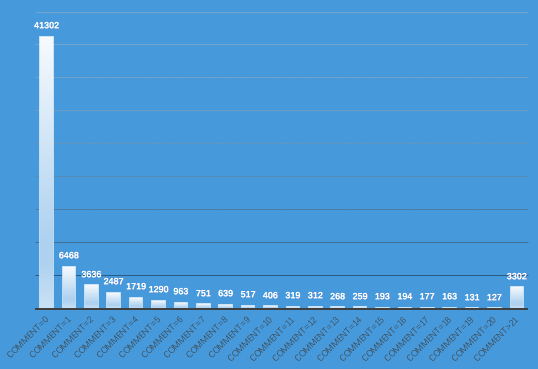
\includegraphics[width=0.99\columnwidth]{comment.png} 
	}
	\subfigure[ ] { \label{fig:b} 
	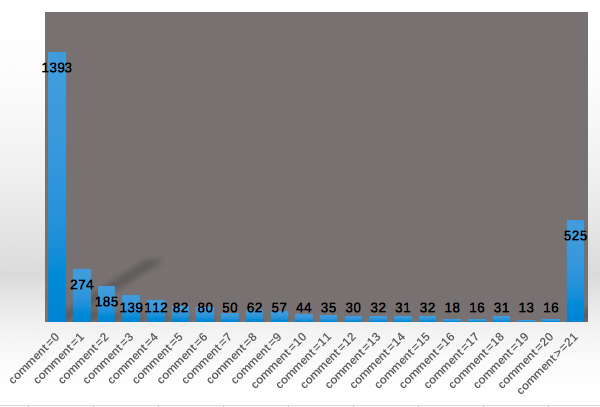
\includegraphics[width=0.99\columnwidth]{comment1.png} 
	}  
	\caption{Comment amount of 3247 overlap russian core users in Stackoverflow}		
\end{figure}

\\65623 Russain users have 559217 comments(average number is 8.522).
 4818 coreusers have 481091 comments(average number is 99.853). And the 60805 users who are not core users have 78126 comments(average number is 1.285).
3247 core users in the overlap set have 395088 comments(average number is 121.678).
1402 core users in the overlap from Stackoverflow main site have 185845 comments(average number is132.558)
some results in figure 15
 \begin{figure}[H]
 		\centering 
	\subfigure[Comments compare between coreusers with  others] { \label{fig:b} 
	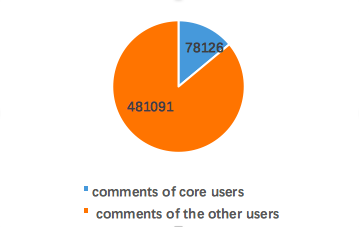
\includegraphics[width=0.7\columnwidth]{commentcompare1.png} 
	}
	\subfigure[Comments compare between migration core users with the other coreusers ] { \label{fig:b} 
	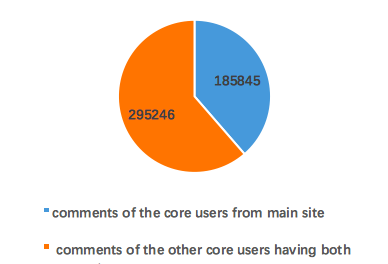
\includegraphics[width=0.7\columnwidth]{commentcompare2.png} 
	}  
	\caption{comments compare}
	\label{fig} 

  	\end{figure}
So the result is the core users from Main site are the most active users in posting comments. And they contributed 33.23\% comments. The average comments number of this group of people is 132.558.
\end{document}
